\subsection{\large{Разработка математической библиотеки}}
\addcontentsline{toc}{subsection}

В главе с проектированием системы приведена абстрактная архитектура математической библиотеки
и описание общих принципов реализации математических методов. Ниже приведем конкретное воплощение этих общих принципов.

Математическая библиотека называется \textbf{nd\_plan} и имеет следующую структуру пакетов
(см. рис.\ref{pic:implementation__math-packages}).

\begin{figure}[H]
	\hspace*{-2.5 cm}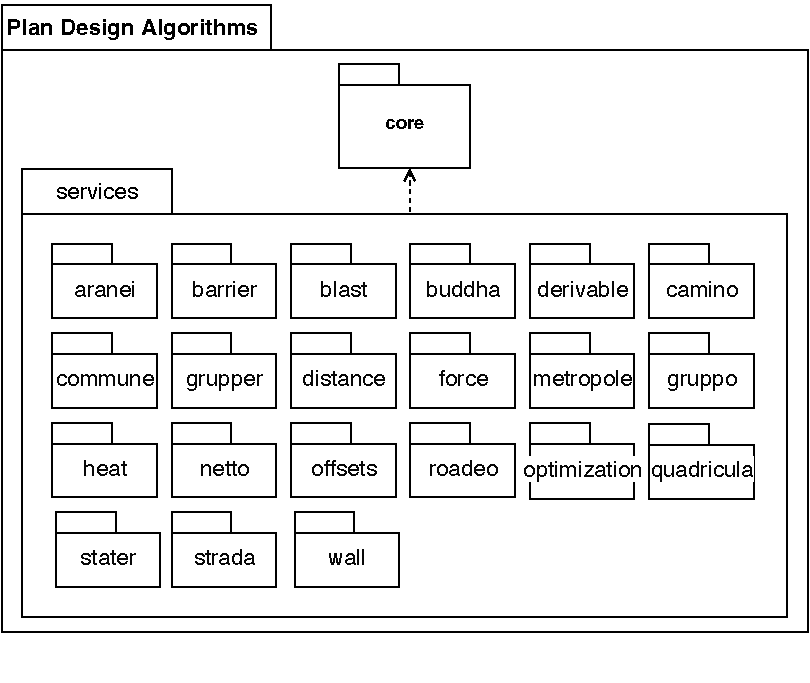
\includegraphics[width=0.7\textwidth]{implementation/pictures/math/packages}
	\caption{Структура пакетов математической библиотеки \textbf{nd\_plan}}
	\label{pic:implementation__math-packages}
\end{figure}
\vskip 5 mm

Пакет \textit{core} содержит методы и классы, которые могут быть свободно переиспользованы.
Каждый пакет расположеннный в пакете \textit{services} это реализация отдельной математической методики.

Приведем пример сервиса, реализующий
методику по расчёту расстояний теплового излучения от факелов. Даннй сервис называется \textit{heat}. Диаграмма классов
данного сервиса изображена ниже (см. рис\ref{pic:implementation__math-classes}).
\begin{figure}[H]
	\hspace*{-2.5 cm}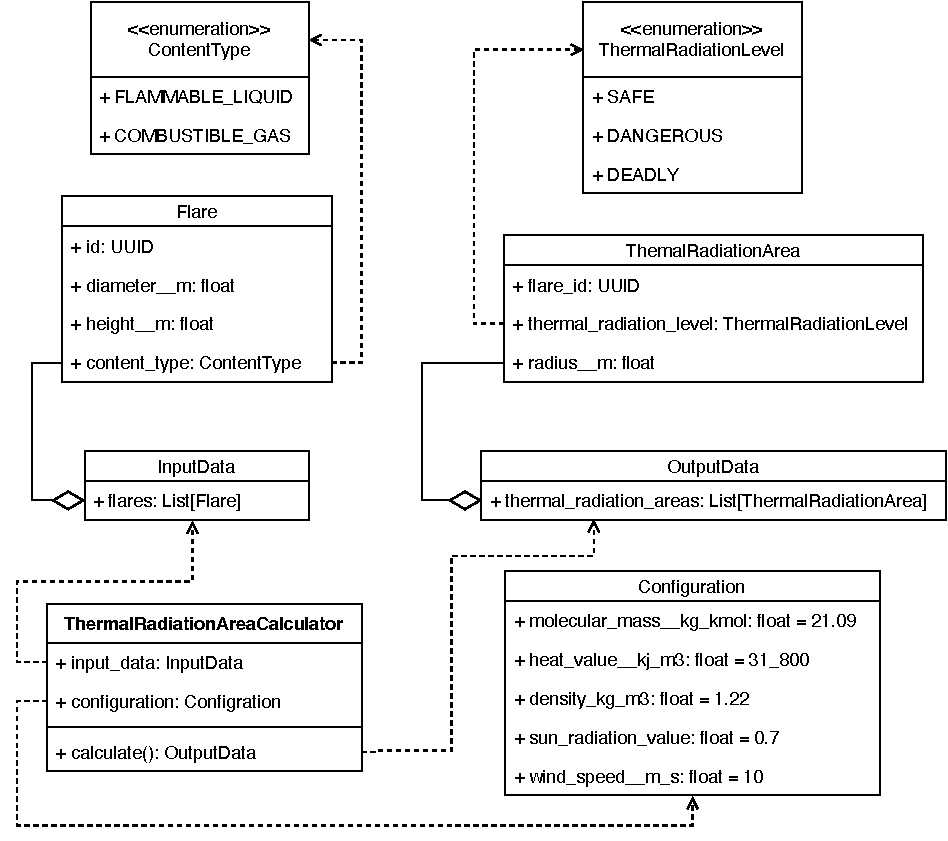
\includegraphics[width=0.9\textwidth]{implementation/pictures/math/classes}
	\caption{Диаграмма классов модели данных сервиса \textbf{heat}}
	\label{pic:implementation__math-classes}
\end{figure}
\vskip 5 mm

Так как мы знаем, что расчет теплового излучения может быть произведен только для факелов, то все сооружения,
используемые в этом сервисе, мы можем сразу же обозначить, как факелы. Название класса \textit{Flare} сразу позволит
понять, с какими объектами оперирует методика, не заглядывая в документацию.